\documentclass[a4paper]{article}
\usepackage{float}
\usepackage[utf8]{inputenc}
\usepackage[T1]{fontenc}
\usepackage{graphicx}
\usepackage[frenchb]{babel}
\usepackage{amsmath}
\usepackage{listings}
\usepackage{hyperref}

% define our color
\usepackage{xcolor}

% code color
\definecolor{ligthyellow}{RGB}{250,247,220}
\definecolor{darkblue}{RGB}{5,10,85}
\definecolor{ligthblue}{RGB}{1,147,128}
\definecolor{darkgreen}{RGB}{8,120,51}
\definecolor{darkred}{RGB}{160,0,0}

% other color
\definecolor{ivi}{RGB}{141,107,185}


\lstset{
    language=scilab,
    captionpos=b,
    extendedchars=true,
    frame=lines,
    numbers=left,
    numberstyle=\tiny,
    numbersep=5pt,
    keepspaces=true,
    breaklines=true,
    showspaces=false,
    showstringspaces=false,
    breakatwhitespace=false,
    stepnumber=1,
    showtabs=false,
    tabsize=3,
    basicstyle=\small\ttfamily,
    backgroundcolor=\color{ligthyellow},
    keywordstyle=\color{ligthblue},
    morekeywords={include, printf, uchar},
    identifierstyle=\color{darkblue},
    commentstyle=\color{darkgreen},
    stringstyle=\color{darkred},
}

\begin{document}

\title{VISA -- TP Segmentation}
\author{Arnaud Cojez}
\date{mercredi 16 novembre 2016}

\maketitle

\newpage
\tableofcontents
\newpage
%----------------------------------------------------------------------------------------
%	INTRODUCTION
%----------------------------------------------------------------------------------------

\section{Introduction}
Nous avons vu dans le précédent TP comment étaient représentées les couleurs en informatique. Dans ce TP, nous allons tenter de segmenter des images par classification de pixels.\\

Nous devrons écrire une Macro ImageJ qui permet de segmenter une image en un nombre donné de classes. Nous segmenterons ensuite d'autres images en utilisant ces classes et observerons les résultats.

\clearpage
%----------------------------------------------------------------------------------------
%	SEGMENTATION DES IMAGES
%----------------------------------------------------------------------------------------
\section{Segmentation des images par K-Means et discrimination linéaire}

\subsection{Explication}
Le but ici est d'écrire une macro qui permet dans un premier temps de segmenter une image en un nombre donné de classes.
Pour ce faire nous utilisons l'algorithme supervisé K-Means grâce au plugin Segmentation > K-Means Clustering fourni.\\

Nous parcourons ensuite l'image Cluster Centroid Values afin de stocker les valeurs RGB des différentes classes.\\

Puis nous demandons à l'utilisateur d'ouvrir une nouvelle image.\\

Ensuite, nous segmentons la nouvelle image en sélectionnant pour chaque pixel la classe dont la couleur est la plus proche de la couleur courante (dans l'espace RGB).

{\em La Macro a été fournie en pièce jointe.}

\subsection{Résultats}
Nous testons dans un premier temps la macro sur l'image {\em cas\_3\_dalton15}, en demandant 6 classes. Nous obtenons l'image segmentée ci-dessous (à droite) ainsi que les valeurs des différentes classes.

\begin{figure}[H]
\begin{center}
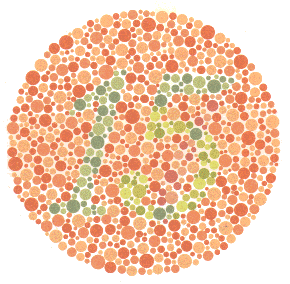
\includegraphics[width=170px]{../base/cas_3_dalton15.png}
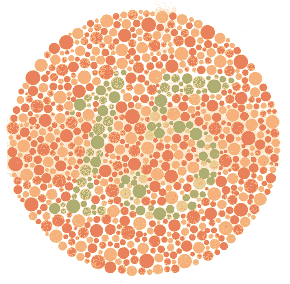
\includegraphics[width=170px]{../resultats/cas_3_dalton15.png}
\end{center}
\caption{À gauche : Image initiale | À droite : Image segmentée}
\end{figure}

\begin{enumerate}
  \item R=255, G=255, B=255
  \item R=252, G=231, B=207
  \item R=247, G=177, B=124
  \item R=234, G=206, B=148
  \item R=233, G=130, B=092
  \item R=174, G=174, B=114
\end{enumerate}

Nous devons maintenant ouvrir une nouvelle image. Nous sélectionnons {\em cas\_3\_dalton74} pour la segmenter selon la méthode citée plus haut. Voici le résultat obtenu.

\begin{figure}[H]
\begin{center}
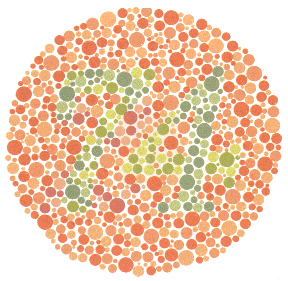
\includegraphics[width=170px]{../base/cas_3_dalton74.png}
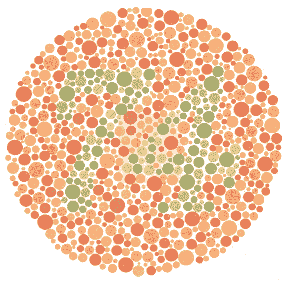
\includegraphics[width=170px]{../resultats/cas_3_dalton74.png}
\end{center}
\caption{À gauche : Image initiale | À droite : Image segmentée}
\end{figure}

\clearpage
%----------------------------------------------------------------------------------------
%	APPLICATION
%----------------------------------------------------------------------------------------
\section{Application aux images cas\_4}

\subsection{Explication}

Le but de cette partie est d'appliquer la macro codée dans la partie précédente et d'observer les résultats sur le lot d'images {\em cas\_4}.\\

La première image selectionnée et segmentée est l'image {\em cas\_4\_dalton6}. Nous utiliserons les 6 classes extraites de cette image afin de segmenter les images suivantes.

\subsection{Résultats}

\subsubsection{Image cas\_4\_dalton6}

Après classification et segmentation par la méthod K-Means, nous obtenons l'image ci-dessous (à droite).

\begin{figure}[H]
\begin{center}
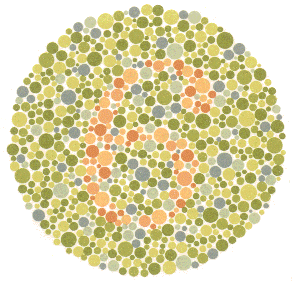
\includegraphics[width=170px]{../base/cas_4_dalton6.png}
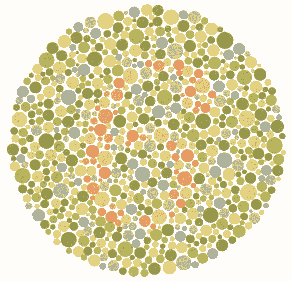
\includegraphics[width=170px]{../resultats/cas_4_dalton6.png}
\end{center}
\caption{À gauche : Image initiale | À droite : Image segmentée}
\end{figure}

Les classes obtenues sont les suivantes :

\begin{enumerate}
  \item R=255, G=255, B=255
  \item R=252, G=231, B=207
  \item R=247, G=177, B=124
  \item R=234, G=206, B=148
  \item R=233, G=130, B=092
  \item R=174, G=174, B=114
\end{enumerate}

Nous observons l'image résultante dans les repères RGB et HSV, grâce au plugin Color Inspector 3D :

\begin{figure}[H]
\begin{center}
  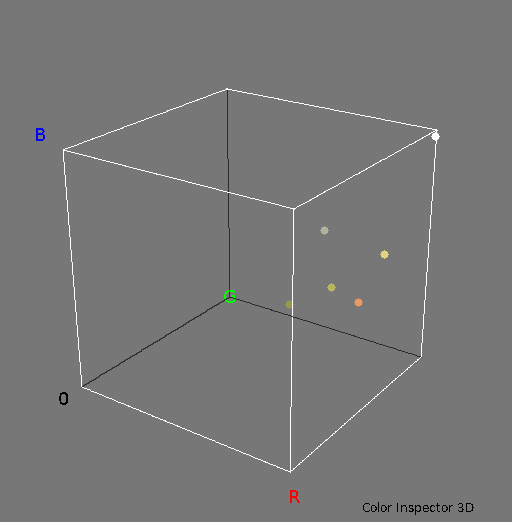
\includegraphics[width=170px]{../resultats/cas_4_dalton6_rgb.png}
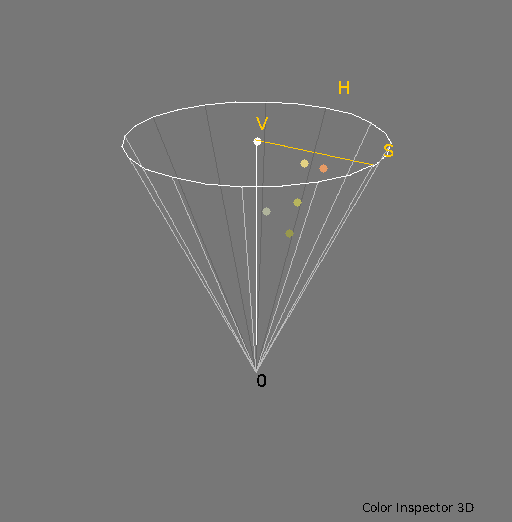
\includegraphics[width=170px]{../resultats/cas_4_dalton6_hsv.png}
\end{center}
\caption{À gauche : Vue dans l'espace RGB | À droite : Vue dans l'espace HSV}
\end{figure}

Nous ne voyons plus que 6 couleurs. Ces couleurs correspondent aux classes trouvées plus tôt. En effet, chaque pixel a pris la couleur de la classe la plus proche dans le repère RGB. D'où ces résultats.

\clearpage
\subsubsection{Image cas\_4\_dalton8}

Après segmentation, nous obtenons l'image suivante :

\begin{figure}[H]
\begin{center}
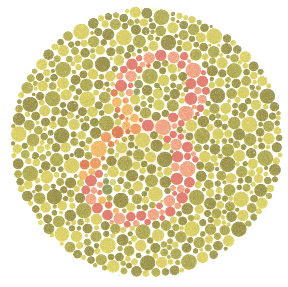
\includegraphics[width=170px]{../base/cas_4_dalton8.png}
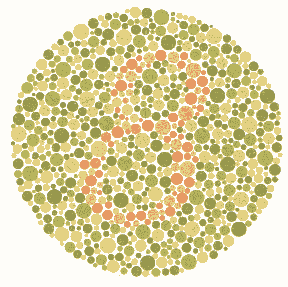
\includegraphics[width=170px]{../resultats/cas_4_dalton8.png}
\end{center}
\caption{À gauche : Image initiale | À droite : Image segmentée}
\end{figure}

Nous observons l'image résultante dans les repères RGB et HSV, grâce au plugin Color Inspector 3D :

\begin{figure}[H]
\begin{center}
  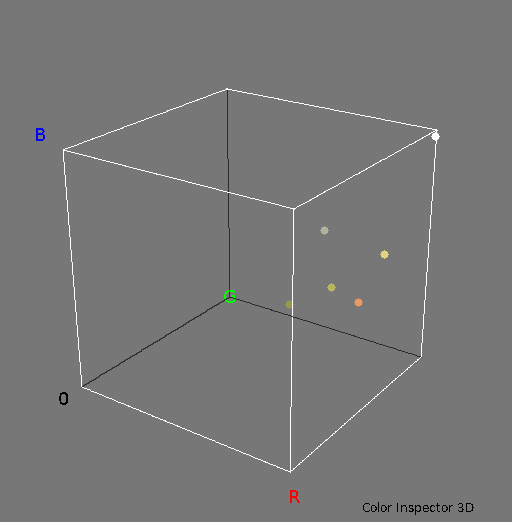
\includegraphics[width=170px]{../resultats/cas_4_dalton8_rgb.png}
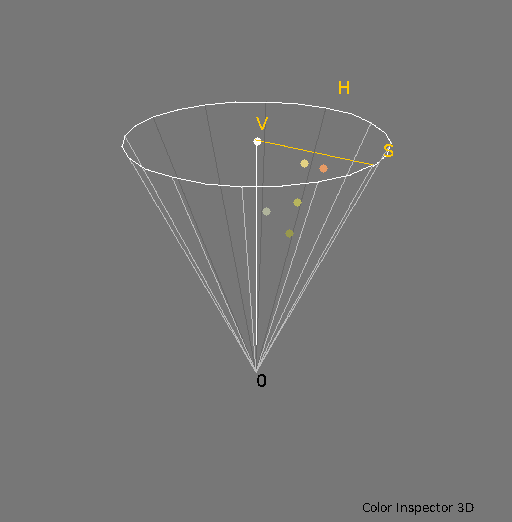
\includegraphics[width=170px]{../resultats/cas_4_dalton8_hsv.png}
\end{center}
\caption{À gauche : Vue dans l'espace RGB | À droite : Vue dans l'espace HSV}
\end{figure}

Ici également, nous voyons seulement 6 couleurs. Ces couleurs correspondent aux classes trouvées plus tôt.

\clearpage
\subsubsection{Image cas\_4\_dalton29}

Après segmentation, nous obtenons l'image suivante :

\begin{figure}[H]
\begin{center}
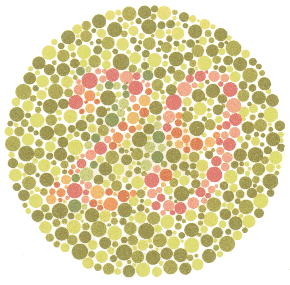
\includegraphics[width=170px]{../base/cas_4_dalton29.png}
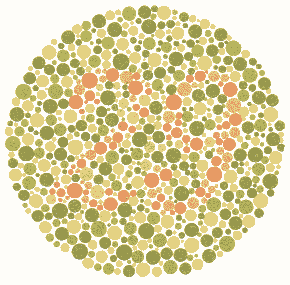
\includegraphics[width=170px]{../resultats/cas_4_dalton29.png}
\end{center}
\caption{À gauche : Image initiale | À droite : Image segmentée}
\end{figure}

Nous observons l'image résultante dans les repères RGB et HSV, grâce au plugin Color Inspector 3D :

\begin{figure}[H]
\begin{center}
  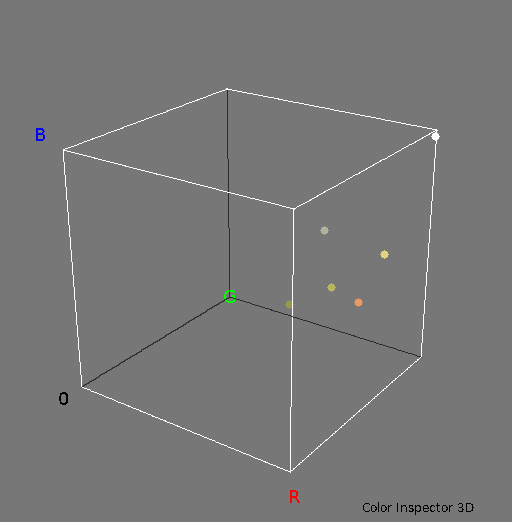
\includegraphics[width=170px]{../resultats/cas_4_dalton29_rgb.png}
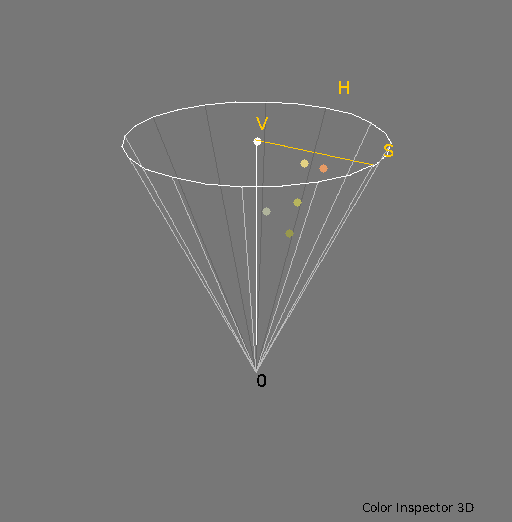
\includegraphics[width=170px]{../resultats/cas_4_dalton29_hsv.png}
\end{center}
\caption{À gauche : Vue dans l'espace RGB | À droite : Vue dans l'espace HSV}
\end{figure}

Ici également, nous voyons seulement 6 couleurs. Ces couleurs correspondent aux classes trouvées plus tôt.

\clearpage
\subsubsection{Image cas\_4\_dalton45}

Après segmentation, nous obtenons l'image suivante :

\begin{figure}[H]
\begin{center}
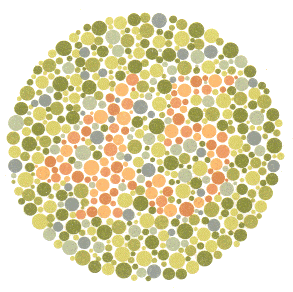
\includegraphics[width=170px]{../base/cas_4_dalton45.png}
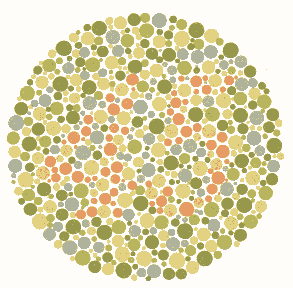
\includegraphics[width=170px]{../resultats/cas_4_dalton45.png}
\end{center}
\caption{À gauche : Image initiale | À droite : Image segmentée}
\end{figure}

Nous observons l'image résultante dans les repères RGB et HSV, grâce au plugin Color Inspector 3D :

\begin{figure}[H]
\begin{center}
  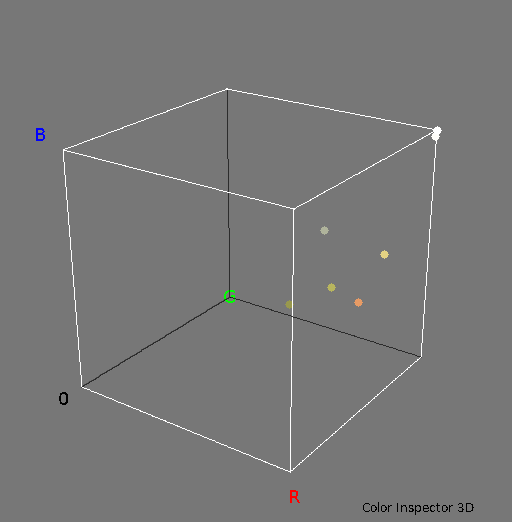
\includegraphics[width=170px]{../resultats/cas_4_dalton45_rgb.png}
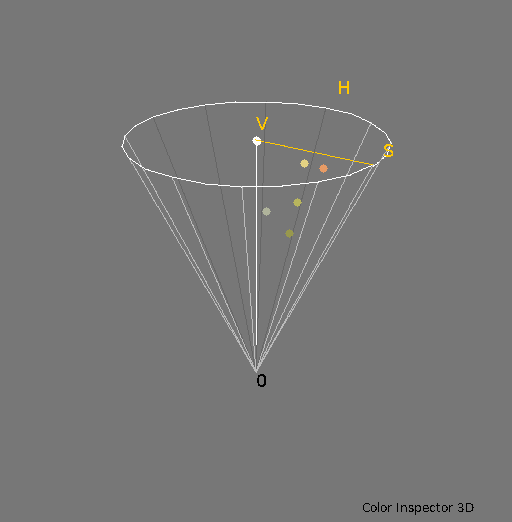
\includegraphics[width=170px]{../resultats/cas_4_dalton45_hsv.png}
\end{center}
\caption{À gauche : Vue dans l'espace RGB | À droite : Vue dans l'espace HSV}
\end{figure}

Ici également, nous voyons seulement 6 couleurs. Ces couleurs correspondent aux classes trouvées plus tôt.

\clearpage
\subsubsection{Image cas\_4\_dalton\_ligne}

Après segmentation, nous obtenons l'image suivante :

\begin{figure}[H]
\begin{center}
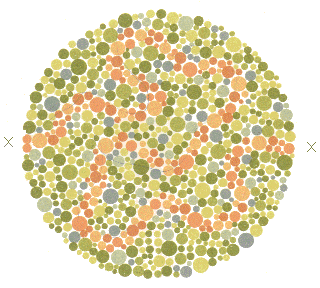
\includegraphics[width=170px]{../base/cas_4_dalton_ligne.png}
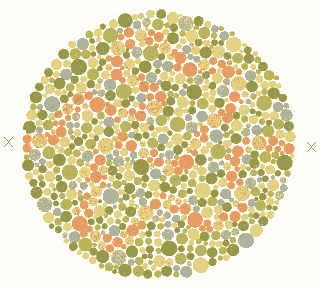
\includegraphics[width=170px]{../resultats/cas_4_dalton_ligne.png}
\end{center}
\caption{À gauche : Image initiale | À droite : Image segmentée}
\end{figure}

Nous observons l'image résultante dans les repères RGB et HSV, grâce au plugin Color Inspector 3D :

\begin{figure}[H]
\begin{center}
  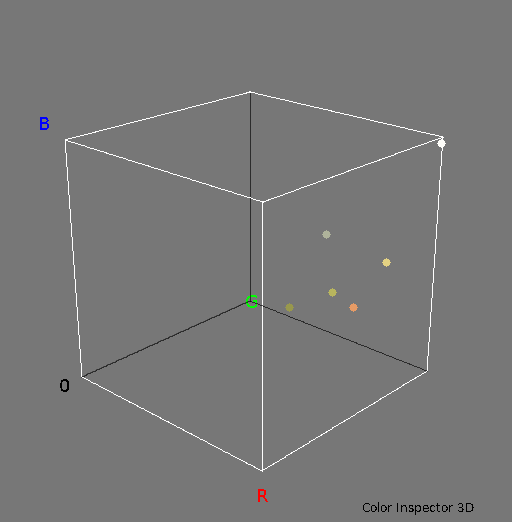
\includegraphics[width=170px]{../resultats/cas_4_dalton_ligne_rgb.png}
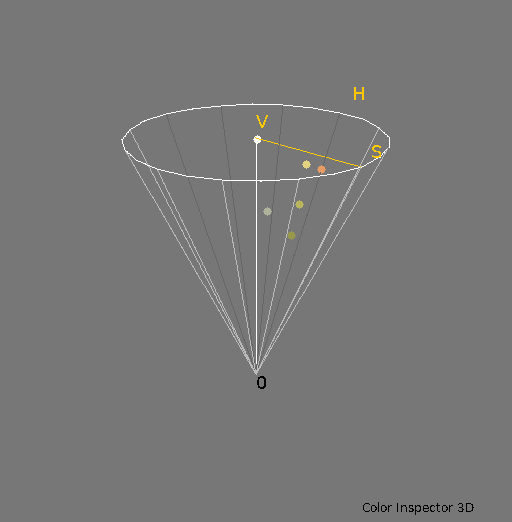
\includegraphics[width=170px]{../resultats/cas_4_dalton_ligne_hsv.png}
\end{center}
\caption{À gauche : Vue dans l'espace RGB | À droite : Vue dans l'espace HSV}
\end{figure}

Ici également, nous voyons seulement 6 couleurs. Ces couleurs correspondent aux classes trouvées plus tôt.

\clearpage
%----------------------------------------------------------------------------------------
%	CONCLUSION
%----------------------------------------------------------------------------------------

\section{Conclusion}
Après avoir défini ce qu'étaient les couleurs et leurs représentations, nous avons pu segmenter des images en utilisant l'algorithme K-Means Clustering.\\

Cet algorithme nous a permis -- une fois spécifié le nombre de classes voulues -- d'obtenir les couleurs de chaque classes. Une fois ces couleurs stockées, nous avons pu segmenter des images similaires en récupérant pour chaque pixel, la classe la plus proche de sa couleur.\\

Nous avons observé que dans les espaces RGB et HSV, il n'y avait plus que les couleurs associées aux classes utilisées pour la segmentation.

\clearpage
%----------------------------------------------------------------------------------------

\end{document}
